\begin{activity} \label{8.1.Act3} Use graphical and/or algebraic methods to determine whether each of the following sequences converges or diverges.
\ba
\item $\left\{\frac{1+2n}{3n-2}\right\}$


\item $\left\{\frac{5+3^n}{10+2^n}\right\}$

\item $\left\{\frac{10^n}{n!}\right\}$ (where $!$ is the \emph{factorial} symbol and $n! = n(n-1)(n-2) \cdots (2)(1)$ for any positive integer $n$ (as convention we define $0!$ to be 1)).

\ea
\end{activity}

\begin{smallhint}
\ba
	\item Small hints for each of the prompts above.
\ea
\end{smallhint}
\begin{bighint}
\ba
	\item Big hints for each of the prompts above.
\ea
\end{bighint}
\begin{activitySolution}
\ba
	\item A plot of the first 50 terms of the sequence $\left\{\frac{1+2n}{3n-2}\right\}$ is shown here.
\begin{center} \resizebox{!}{1.75in}{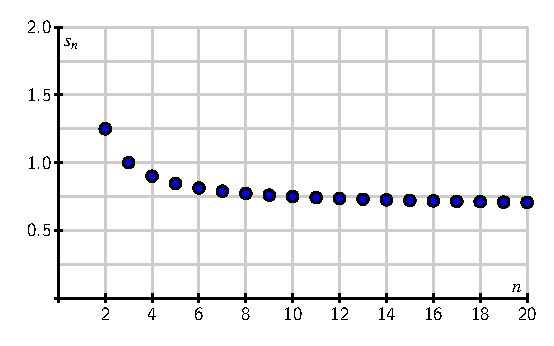
\includegraphics{figures/8_2_Sequence_a.eps}} \end{center}
The plot implies that the sequence has a limit between 0.5 and 1. For large $n$ the $2n$ term dominates the numerator and the $3n$ term the denominator. So $\frac{1+2n}{3n-2}$ looks like $\frac{2n}{3n} = \frac{2}{3}$ when $n$ is big. So the sequence $\left\{\frac{1+2n}{3n-2}\right\}$ converges to $\frac{2}{3}$.
    \item A plot of the first 50 terms of the sequence $\left\{\frac{5+3^n}{10+2^n}\right\}$ is shown here.
\begin{center} \resizebox{!}{1.75in}{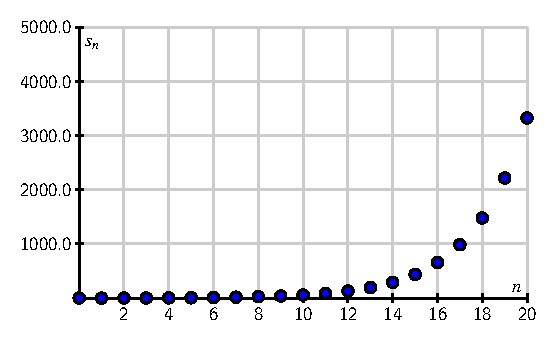
\includegraphics{figures/8_2_Sequence_b.eps}} \end{center}
The plot implies that the sequence does not have a limit as $n$ goes to infinity. For large $n$ the $3^n$ term dominates the numerator and the $2^n$ term the denominator. So $\frac{5+3^n}{10+2^n}$ looks like $\frac{3^n}{2^n} = \left(\frac{3}{2}\right)^n$ when $n$ is big. Since $\frac{3}{2} > 1$, the sequence $\left\{\frac{5+3^n}{10+2^n}\right\}$ diverges to infinity.
    \item A plot of the first 50 terms of the sequence $\left\{\frac{10^n}{n!}\right\}$ is shown here.
\begin{center} \resizebox{!}{1.75in}{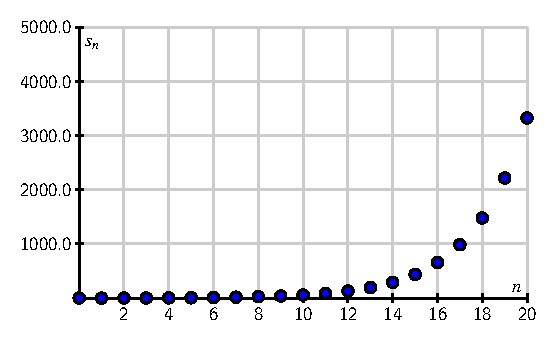
\includegraphics{figures/8_2_Sequence_b.eps}} \end{center}
Initially, it looks as though the terms increase without bound, but beginning at about $n=10$ the factorial in the denominator dominates the numerator. Notice that
 \[\frac{10^n}{n!} = \frac{10 \times 10 \times 10 \times \cdots \times 10}{1 \times 2 \times 3 \times \cdots n}\]
When $n > 20$, we have that $\frac{10}{n} < \frac{1}{2}$ and 
\begin{align*}
\frac{10^n}{n!} &= \left(\frac{10 \times 10 \times 10 \times \cdots \times 10}{1 \times 2 \times 3 \times \cdots 20}\right) \left(\frac{10 \times 10 \times 10 \times \cdots \times 10}{21 \times 22 \times 23 \times \cdots n}\right) \\
    &= \left(\frac{10^{20}}{20!}\right) \left(\frac{10}{21}\right) \left(\frac{10}{22}\right) \cdots \left(\frac{10}{n}\right)  \\
    &< \left(\frac{10^{20}}{20!}\right) \left(\frac{1}{2}\right)^{n-20}.
\end{align*}
Since $\frac{1}{2}<1$, the term $\left(\frac{1}{2}\right)^{n-20}$ goes to 0 as $n$ goes to infinity. The fact that $\frac{10^{20}}{20!}$ is a constant means that $\frac{10^n}{n!} \to 0$ as $n \to \infty$. 

\ea
\end{activitySolution}
\aftera 